% Chapter 3

\chapter{REQUIREMENTS ANALYSIS} % All Chapter Headings in ALL CAPS

\section{FUNCTIONAL REQUIREMENTS}
 The system recommends the best service for the given set of services.The output should adheere to the following requirements:
\begin{itemize}
  \item The service should be recommended based on the qos values
  \item The recommended service should be based on the location of the user
  \item The system must be optimized
  \item The system should predict the qos values based on the past experience of the user
   \item The system should not predict the qos values for the untrusted user
\end{itemize}  
\section{NON FUNCTIONAL REQUIREMENTS}
\subsection{User Interface}
 There must be a simple and easy to use user interface where the user
should be able to use their web service. The qos values predicted and
also the recommended service should be displayed in the screen.
\subsection{Hardware}
  No special hardware interface is required for the successful imple-
mentation of the system.
\newpage
\subsection{Software}
\begin{itemize}
    \item Operating System:Windows
    \item Programming language:JAVA
    \item Database:HeidiSQL
    \item Tools:NetBeans IDE, WAPT
\end{itemize}
\subsection{Performance}
  The system must be optimized, reliable, consistent and available
  all the time.
\section{CONSTRAINTS AND ASSUMPTIONS}
\subsection{Constraints}
\begin{itemize}
    \item The system will predict the qos values only for the trusted users
    \item The dataset considered will be based on the usage of the users who utilized that service
    \item The web service should be error free
    \item The recommendation will be based on the experience of the co-users who have used that service
    
\end{itemize}
\subsection{Assumptions}
\begin{itemize}
    \item The qos values provided by the new user for a new web service will be considered as trust worthy 
    \item The outputs provided by the WAPT tool will be taken as a part of input
\end{itemize}
\bigskip
\bigskip
\section{SYSTEM MODELS}
\subsection{Overall Use Case Diagram}

 The overall usecase diagram of the entire system is shown in figure
3.1. It consists of recommendation processes.
\begin{figure}[h!]
  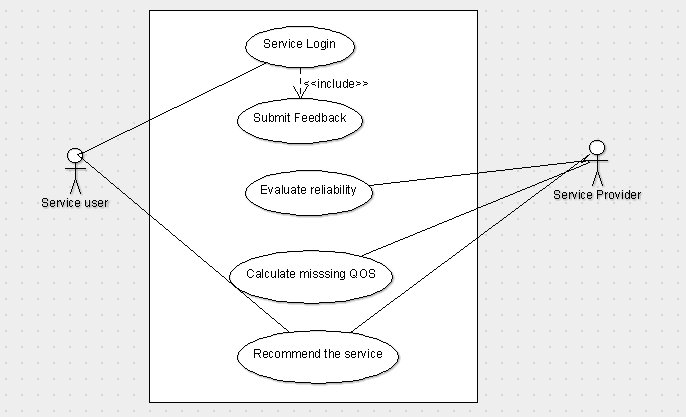
\includegraphics[scale=0.7]{overuse}
  \caption{Overall Use Case Diagram}
  \label{fig:boat1}
\end{figure}

\linebreak
\textbf{Description}: The system finds the reliability of the users based on the QOS values. Also it calulates the QOS values missed by the users based on their past experience. Then the location of the user is being considered and then the best service will be recommended.

\\*\textbf{Pre condition}: The web services are created and utilised by the user

\\*\textbf{Post condition}: The best service is recommended to the user based on parameters.
\newpage
\subsection{Reliability Evaluation-Use Case Diagram }
 The usecase diagram of reliability evaluation is shown in figure 3.2. It consists of handling the input and finding the reliability of the user.
 
\begin{figure}[h!]
\centering
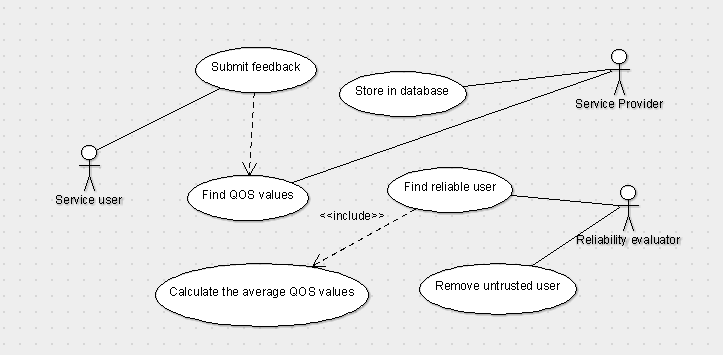
\includegraphics[scale=0.7]{reluse}
\caption{Reliability Use Case Diagram}
\label{fig:universe}
\end{figure}

\textbf{Description}: The QOS feedbacks from the service consumers are collected in the input handler and then stored in the DataSet.
These datasets are collaborated and send as an input for Reliability calculation and then QOS prediction.They include QOS values for various services from various users. As not every users are reliable ones, we eliminate the QOS values of untrusted users and then provide with best results. A user is considered to be trusted based on the frequency of usage, the contract duration, and the threshold on the number of users. Also, the users who give ratings as all are best are also eliminated.

\\*\textbf{Pre condition}: The web services are invoked by the user and feedback is provided.

\\*\textbf{Post condition}: The input provided are saved and the reliability of the user is predicted. 

\bigskip
\subsection{Recommendation-Use Case Diagram }
 The usecase diagram of recommendation is shown in figure 3.3. It consists of finding the missing QOS values and recommending the web service to the user.

\bigskip
\textbf{Description}:Not every users could provide the correct feedbacks and not every user is reliable. This section takes care of Missing QOS values based on the Historical values provided and then predicts what  the user could have provided if he had used the system. This section will improve accuracy of recommendation of services. Based on the interest of the users on the services and also based on the location of the users, the services with the best QOS values are recommended. And also the justification for the recommendation is also  provided. This could be also useful for the Service providers to enhance their quality.

\linebreak
\textbf{Pre condition}: The reliability of the user is calculated.

\linebreak
\begin{figure}[h!]
\centering
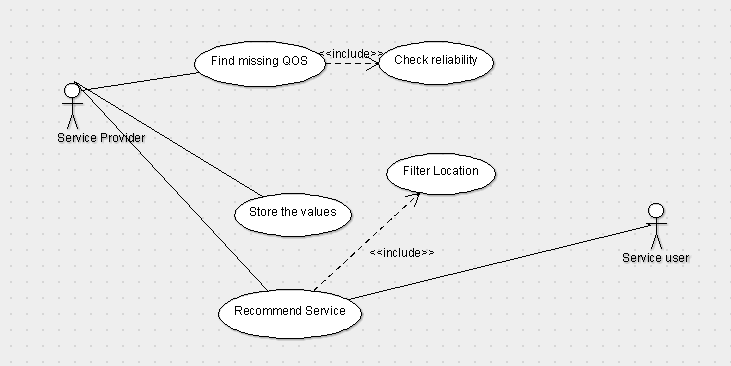
\includegraphics[scale=0.7]{recuse}
\caption{Recommendation Use Case Diagram}
\label{fig:universe}
\end{figure}
\textbf{Post condition}: The QOS values missed by the user are calculated and the web services are recommended. 
\subsection{Reliability Evaluation-Sequence Diagram}
 The sequence diagram of the reliability evaluation is shown in figure 3.4. It can be seen that input handler and reliability evaluator are the main components involved.

\begin{figure}[h!]
\centering
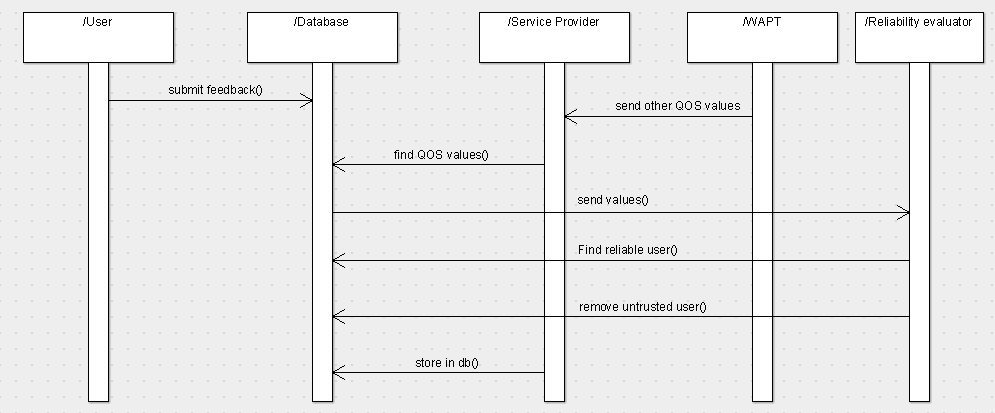
\includegraphics[scale=0.5]{relseqq}
\caption{Reliability Evaluation Sequence Diagram}
\label{fig:universe}
\end{figure}
\linebreak
\subsection{Recommendation-Sequence Diagram}
 The sequence diagram of the recommendation is shown in figure 3.5. It can be seen that missing QOS value predictor, location filtrator are the main components involved.
 \\*
\begin{figure}[h!]
\centering
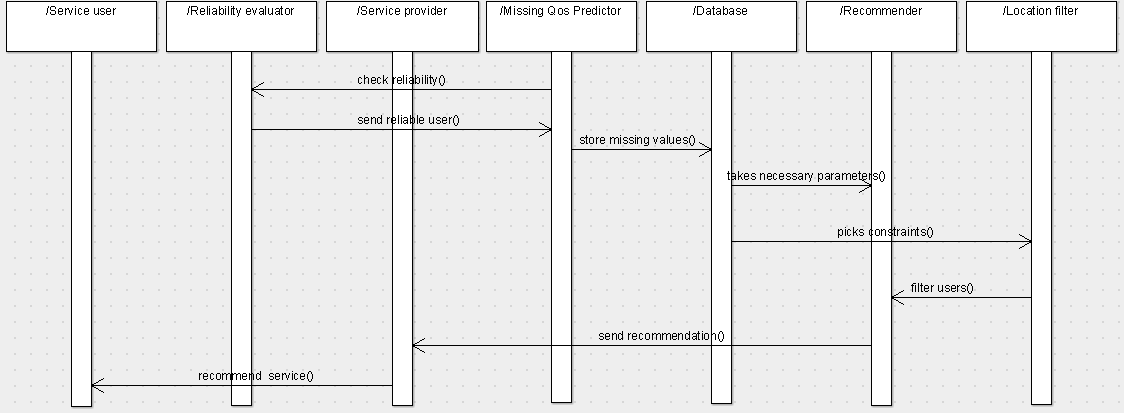
\includegraphics[scale=0.5]{recseqq}
\caption{Recommendation Sequence Diagram}
\label{fig:universe}
\end{figure}
